\lstnewenvironment{Code03_01}[1][]{ \lstset{showspaces=false, showtabs=false,tabsize=2,basicstyle=\small\ttfamily, columns=fullflexible,framexrightmargin=+.1\textwidth, keywordstyle=\color{red}\bfseries, commentstyle=\color{blue},language=C++, basicstyle=\small,  numberstyle=\tiny, stepnumber=1, numbersep=5pt, frame=shadowbox, #1}}{}


\chapter{Considerazioni preliminari}

\section{Strumenti di sviluppo}
Lo sviluppo del nostro progetto ha richiesto l'uso di strumenti specifici atti a facilitare e sistematizzare la gestione del codice quali \texttt{git}, \texttt{CMake} e \texttt{Dxygen}.\\

\subsection{\texttt{Git}}
\href{https://github.com/}{\texttt{Git}} è un sistema di controllo versione utilizzabile direttamente da linea di comando, molto diffuso è utile per tenere traccia delle varie fasi di sviluppo del codice. Git gestisce in modo adeguato i contributi al codice provenienti da agenti esterni e permette la condivisione del codice.\\
Il codice del progetto è reperibile su \texttt{git} ed è possibile scaricarlo e collabolare allo sviluppo clonando il codice dalla repository  \href{https://github.com/}{\texttt{GitHub}}:\\
\begin{center}
\texttt{ git clone https://github.com/mariaiemoli/progetto.git}
\end{center}
Nella cartella principale è contenuto anche un file \texttt{.gitignore}, in cui sono specificate le estensioni dei files e le sottocartelle che non devono essere visionati in una repository \texttt{git}. In particolare non si è interessati ai files temporanei che vengono eventualmente generati dagli editor, e alle cartelle generate da uno scorretta configurazione di \texttt{Doxygen}.

\subsection{\texttt{CMake}}
\href{http://www.cmake.org/}{\texttt{CMake}} è un software libero multipiattaforma nato per l'automazione dello sviluppo. Sostanzialmente con l'uso di \texttt{CMake} è possibile configurare e generare Makefile per il sistema operativo in uso. Questo facilita la diffusione del codice tra sviluppatori, non dovendo far altro che lanciare \texttt{CMake} e lasciare che sia lui ad occuparsi della ricerca di compilatori e librerie locali e della costruzione di software.\\
\texttt{CMake} si basa sulla creazione di files \texttt{CMakeLists.txt} nella directory del progetto, che contengono le direttive necessarie per creare il \texttt{Makefile} per compilare ed eseguire il codice. \\
Nella directory principale si trova un primo file \texttt{CMakeLists.txt} in cui si impostano i parametri fondamentali quali la dipendenza dalla versione di \texttt{CMake}, il nome del progetto, si includono le directory dei sorgenti nel path di compilazione e si caricano le librerie esterne utilizzate dai sorgenti. \\
le librerie che vengono caricate sono:
\begin{enumerate}
\item[-] \texttt{Eigen}, libreria template per l'algebra lineare usata principalmente nella fase di imposizione delle condizioni di interfaccia sul triangolo di intersezione nel caso della biforcazione, per il modello ridotto;
\item[-] \texttt{Getfem++}, libreria matematica per gli elementi finiti usata per scrivere e risolvere il problema numerico;
\item[-] \texttt{Blas} (Basic Linear Algebra Subprograms) e \texttt{Qhull}, librerie necessarie per \texttt{Getfem++};
\item[-] \texttt{Doxygen}, usato per generare la documentazione
\end{enumerate}

\begin{Code03_01}
CMAKE_MINIMUM_REQUIRED( VERSION 2.8 )

PROJECT(PACS)

SET(CMAKE_CXX_FLAGS "-std=c++0x -Wall ${CMAKE_CXX_FLAGS}")

SET(CMAKE_MODULE_PATH 
	${CMAKE_SOURCE_DIR}/cmake ${CMAKE_MODULE_PATH})

# Include Eigen3
FIND_PACKAGE(PkgConfig)
PKG_CHECK_MODULES(EIGEN3 REQUIRED eigen3)
INCLUDE_DIRECTORIES(${EIGEN3_INCLUDE_DIRS})

# Include Doxygen
find_package(Doxygen)
[ ... ]

# Include Getfem
if (GETFEM_LIBRARIES AND GETFEM_INCLUDE_DIRS)
[ ... ]

#Include for BLAS library
find_package ( BLAS )
[ ... ]


#Include for LAPACK library
find_package ( LAPACK )
[ ... ]

#Include for QHULL library
set(QHULL_MAJOR_VERSION 6)
[ ... ]

SET(CMAKE_INSTALL_PREFIX 
${CMAKE_SOURCE_DIR}/install-dir CACHE PATH "" FORCE)

ADD_SUBDIRECTORY(src)
ADD_SUBDIRECTORY(test)
\end{Code03_01}

%% $

Per poter usare \texttt{CMake} è necessario posizionarsi nella directory in cui è contenuto il progetto e creare una cartella in cui compilare il codice. Per lanciare \texttt{CMake} è necessario digitare i seguenti comandi: \\ 

\par  \texttt{cd $<$build\_dir$>$ } 
\par \texttt{cmake $<$source\_dir$>$}\\

\noindent \texttt{CMake} imposta le variabili di path come definito nel file  \texttt{CMakeLists.txt}, esamina le dipendenze da librerie esterne e procede esaminando le sottocartelle aggiunte nel file di configurazione. In particolare esamina le sottocartelle \texttt{src} e \texttt{test}, in cui sono presenti altri files  \texttt{CMakeLists.txt}, che impostano i rispettivi obiettivi e definiscono le rispettive sottocartelle. Questo permette a \texttt{CMake} di esaminare tutta la directory in cui è contenuto il progetto in maniera ricorsiva. \\
%Nella cartella \texttt{src} il file  \texttt{CMakeLists.txt} aggiunge la creazione di una libreria a partire dal codice del progetto. \\
%\begin{Code03_01}
%ADD_LIBRARY(pacs ${TARGET_SRC} ${TARGET_HANDLER})
%\end{Code03_01}

\par \noindent Nella cartella test si trovano delle sottocartelle ognuna delle quali contenente un file data di esempio per poter eseguire il codice e un file  \texttt{CMakeLists.txt} . Il file  \texttt{CMakeLists.txt} nella cartella dei test definisce gli obiettivi e i collegamenti necessari per l'esecuzione. 

\par Una volta che il \texttt{Makefile} è stato generato è possibile compilare il codice con il comando: \\ 
\par \texttt{make}\\

\noindent Questo crea in ogni sottocartella della cartella \texttt{test} un eseguibile chiamato \texttt{Test}. Per poterlo eseguire è sufficiente lanciare da terminale, dopo essersi posizionati nella directory corretta, 
\par \texttt{ .\textbackslash Test-iesimo }

\subsection{\texttt{Doxygen}}
\href{www.doxygen.org/}{\texttt{Doxygen}} è un sistema multipiattaforma molto diffuso per la generazione automatica della documentazione di un codice. Per ottenere la documentazione è necessario introdurre nel codice dei commenti con una sintassi particolare, e il risultato contiene l’elenco delle classi implementate, i loro diagrammi di collaborazione e la descrizione di metodi ed attributi.
Per poter creare la documentazione al codice con \texttt{Doxygen} è necessario che nella cartella principale sia presente il file \texttt{Doxygen}, in caso contrario è necessario crearlo con il comando:\\
\par \texttt{Doxygen -g}\\

\noindent In questo file sono definite le variabili che permettono di creare la documentazione come il nome del progetto, la directory dove creare la documentazione, le cartelle dove si trovano i sorgenti e l'estensione dei files da considerare.

\begin{Code03_01}
PROJECT_NAME 				=	 Problema di Darcy in un network di fratture
OUTPUT_DIRECTORY			=	./build/doc
INPUT						= 	./src ./test
FILE_PATTERNS				= 	*.cc *.h
HAVE_DOT					=	YES
COLLABORATION_GRAPH		=	YES
HIDE_UNDOC_RELATIONS		=	NO
\end{Code03_01}

\noindent Dopo aver lanciato \texttt{CMake} è possibile generare la documentazione semplicemente eseguendo: \\
\par \texttt{cd $<$build\_dir$>$} 
\par \texttt{make doc} \\

\noindent Questo crea una sottocartella \texttt{build/doc} che contiene la documentazione \texttt{html} e \LaTeX{}.

\newpage

\section{Dati del problema}

\subsection{Intersezioni}
Come è stato precedentemente detto, il codice di partenza trattava un tipo particolare di intersezione tra fratture, da noi chiamato \textit{Cross}. Questo tipo di intersezione ha la seguente forma:

\begin{figure}[htbp]
\begin{center}
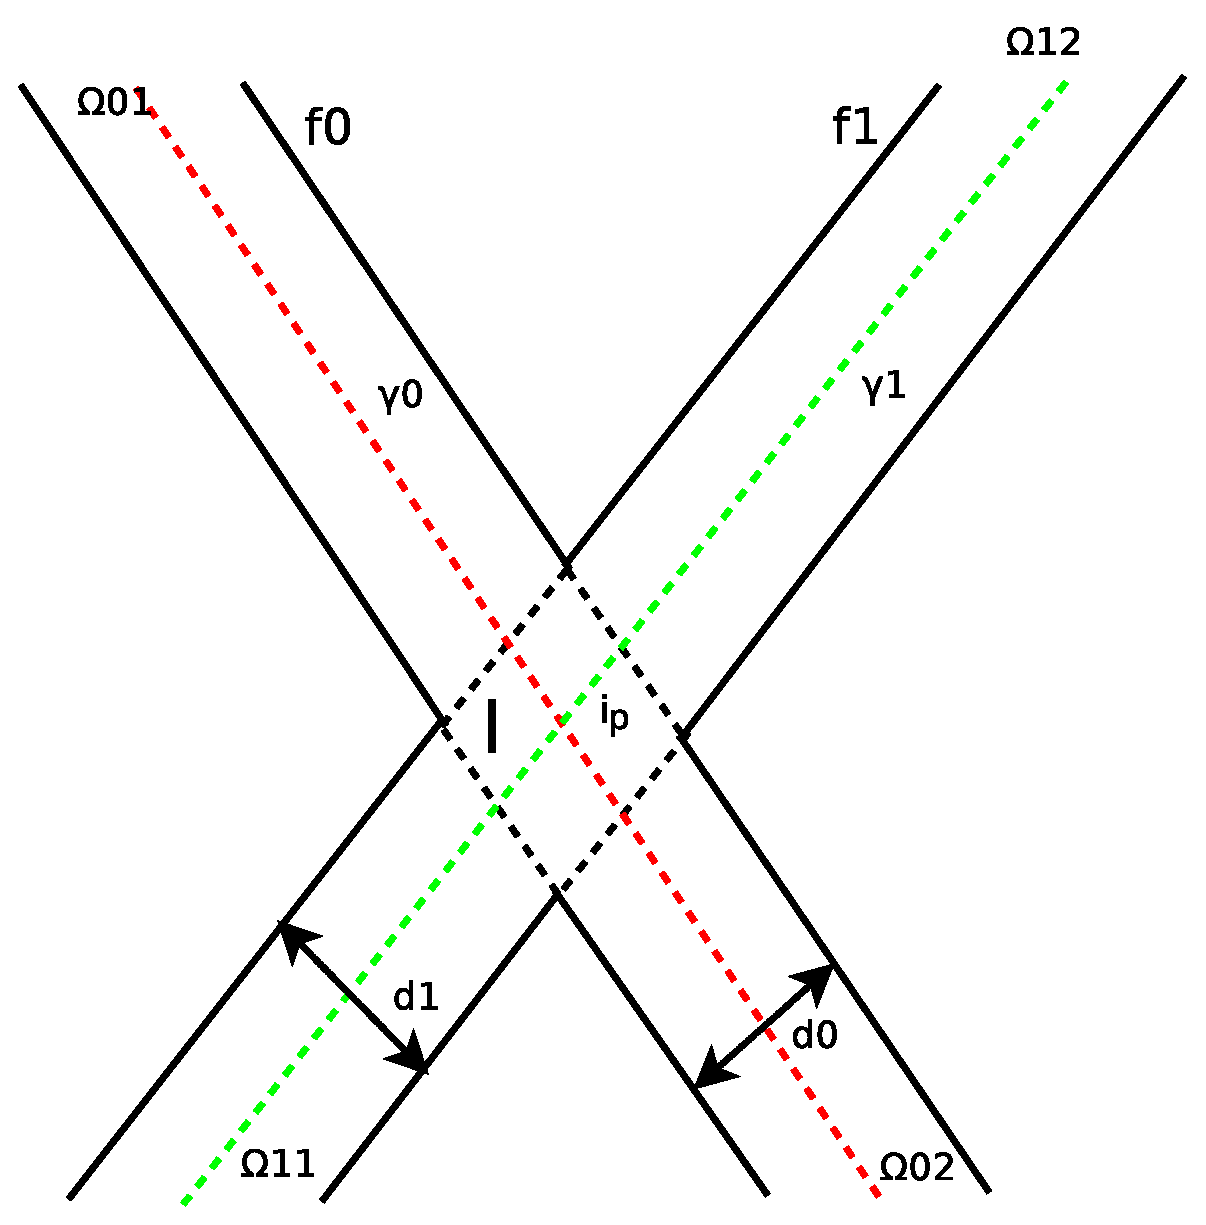
\includegraphics[width=0.4\textwidth]{img/cap2/cross.eps}
\caption{Struttura di un'intersezione di tipo \textit{Cross} tra due fratture.}\label{Cross}
\end{center}
\end{figure}

\noindent L'area di intersezione è constituita da un parallelogramma che suddivide ogni frattura in due zone $\Omega_{i1}$ e $\Omega_{i2}$. Il modello su cui noi ci basiamo riduce la frattura, qui rappresentata in un dominio $\mathbb{R}^{2}$, alla retta di sostegno $\gamma_i$. In questo modo l'intersezione si riduce ad un punto.\\
Il tipo di intersezione su cui ci siamo concentrate noi, invece, ha la seguente forma:

\begin{figure}[htbp]
\begin{center}
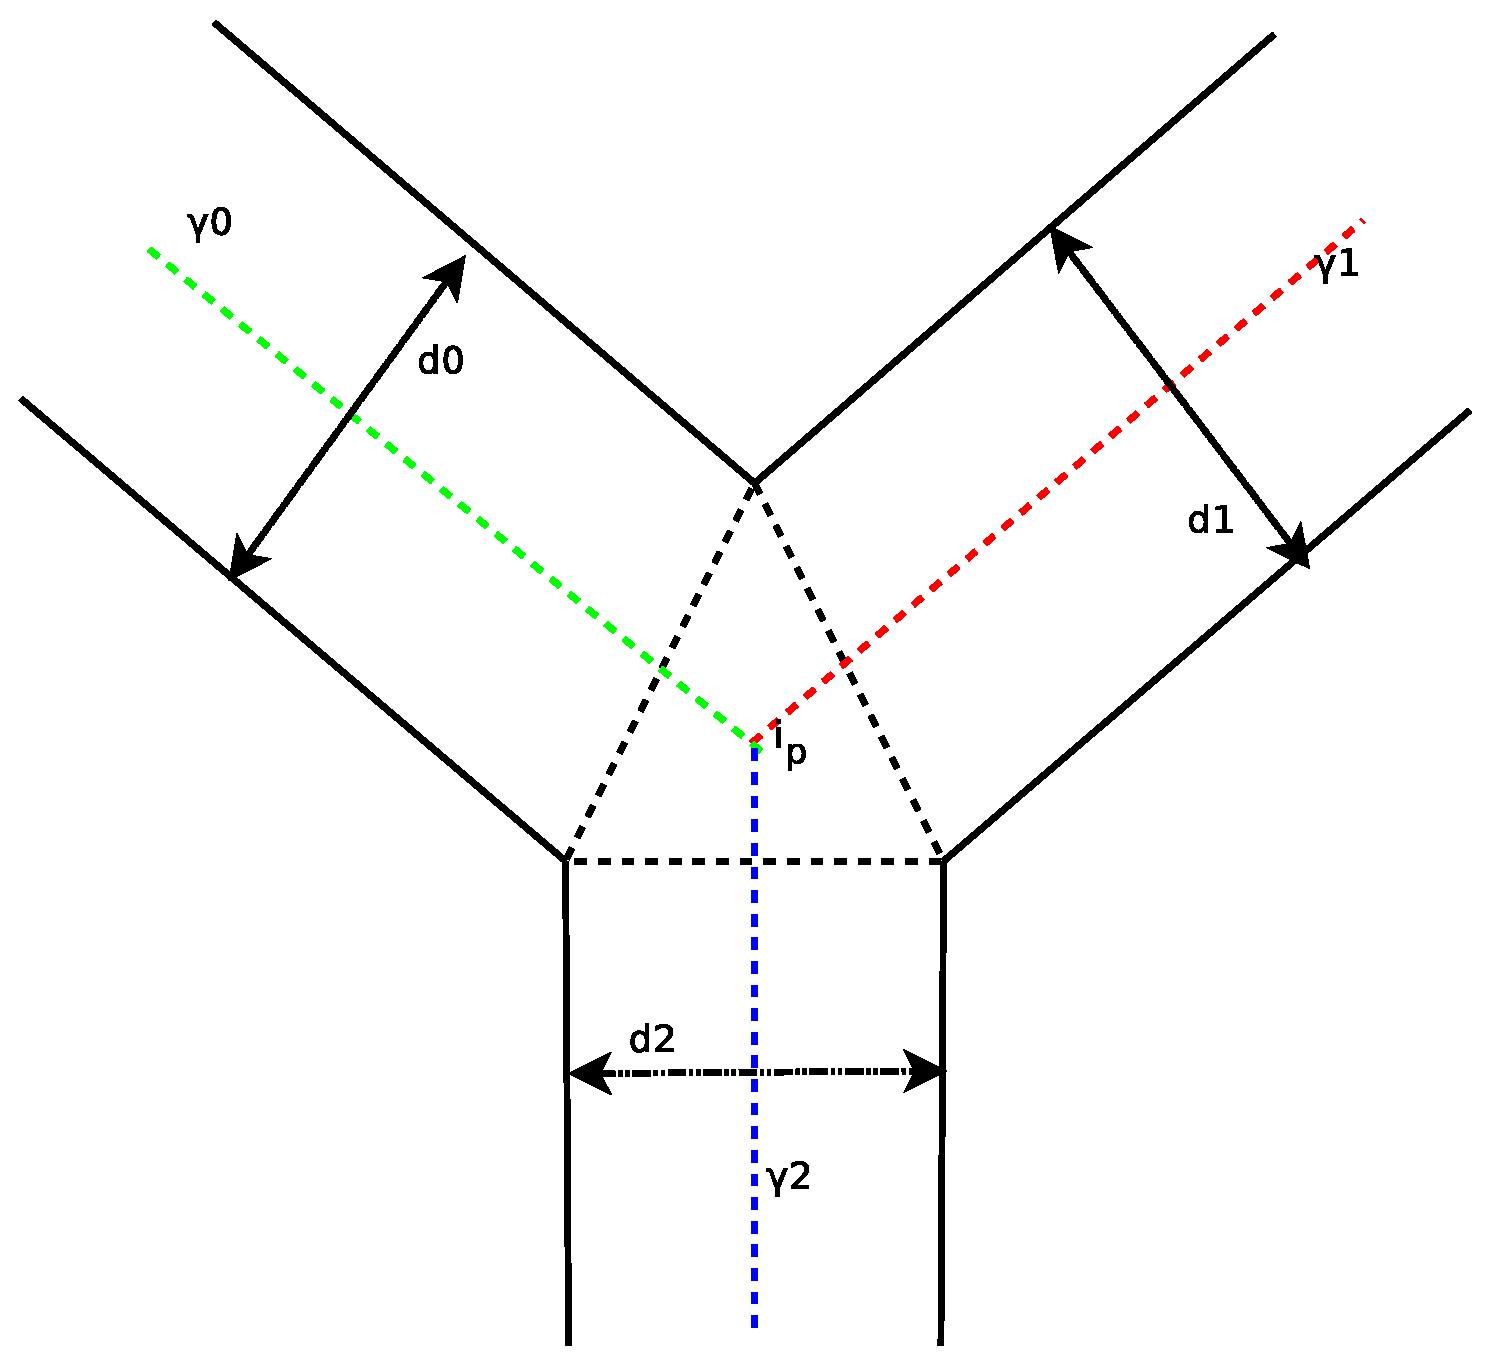
\includegraphics[width=0.4\textwidth]{img/cap2/bifurcation.eps}
\caption{Struttura di un'intersezione di tipo \textit{Bifurcation} tra due fratture.}\label{Bifurcation}
\end{center}
\end{figure}

\noindent In questo caso le fratture coinvolte sono tre e la zona interessata dall'intersezione è rappresentata da un triangolo. Anche qui consideriamo un modello ridotto e le fratture sono individuate dalle rette di sostegno $\gamma_i$ in $\mathbb{R}$. Le condizioni d'interfaccia che vengono ricavate in questo caso valgono solo nel caso in cui le tre fratture si intersechino in un unico punto comune $i_p$ e tale punto sia contenuto nel triangolo d'intersezione nella rappresentazione 2d.

\subsection{File data}

I dati per la definizione del problema sono definiti nei file .txt contenuti nella sottocartella \texttt{dati}. \\
\noindent Ognuno di questi files ha la seguente struttura:

\begin{enumerate}
\item[-] una prima parte dove vengono definite la directory dove trovare l'eventuale mesh da importare, la directory dove salvare i risultati e il numero di fratture che entrano in gioco;
\item[-] una sezione dedicata a parametri e grandezze necessari per la definizione del dominio del mezzo;
\item[-] una sezione per ogni frattura con la dichiarazione del level set, dei parametri che individuano il segmento che rappresenta la frattura e delle grandezze necessarie per risolvere il problema di Darcy.
\end{enumerate}

\begin{Code03_01}[caption={Definizione del dominio}]
meshFile = meshes/mesh		//   directory da cui importare eventualmente la mesh
folderVTK = ./vtk/				//   directory dove salvare i risultati

numberFractures = 3

[mediumData]					//   informazioni legate al mezzo poroso in questione

   [./domain]					//   informazioni necessarie per costruire o importare la mesh 
     [ ... ]
   [../]

   [./darcy]					//   informazioni sulla natura permeabile del mezzo
     invK = 1.
     invKDist11 = 1.
     invKDist12 = 0.
     invKDist22 = 1.
     [...]	
   [../]

[../]

\end{Code03_01}

\par \noindent Nonostante il nostro problema si concentri solamente sulla soluzione del flusso all'interno delle fratture, noi costruiamo comunque la mesh relativa al mezzo. Questa mesh verrà usata solamente come supporto, sarà puramente accessoria nel corso dell'implementazione. \\
 \noindent Per quanto riguarda la permeabilità, poichè le fratture sono costituite dallo stesso materiale, questa resta uguale in tutto il dominio, sia nel mezzo che nelle fratture. 

\begin{figure}[htbp]
\begin{center}
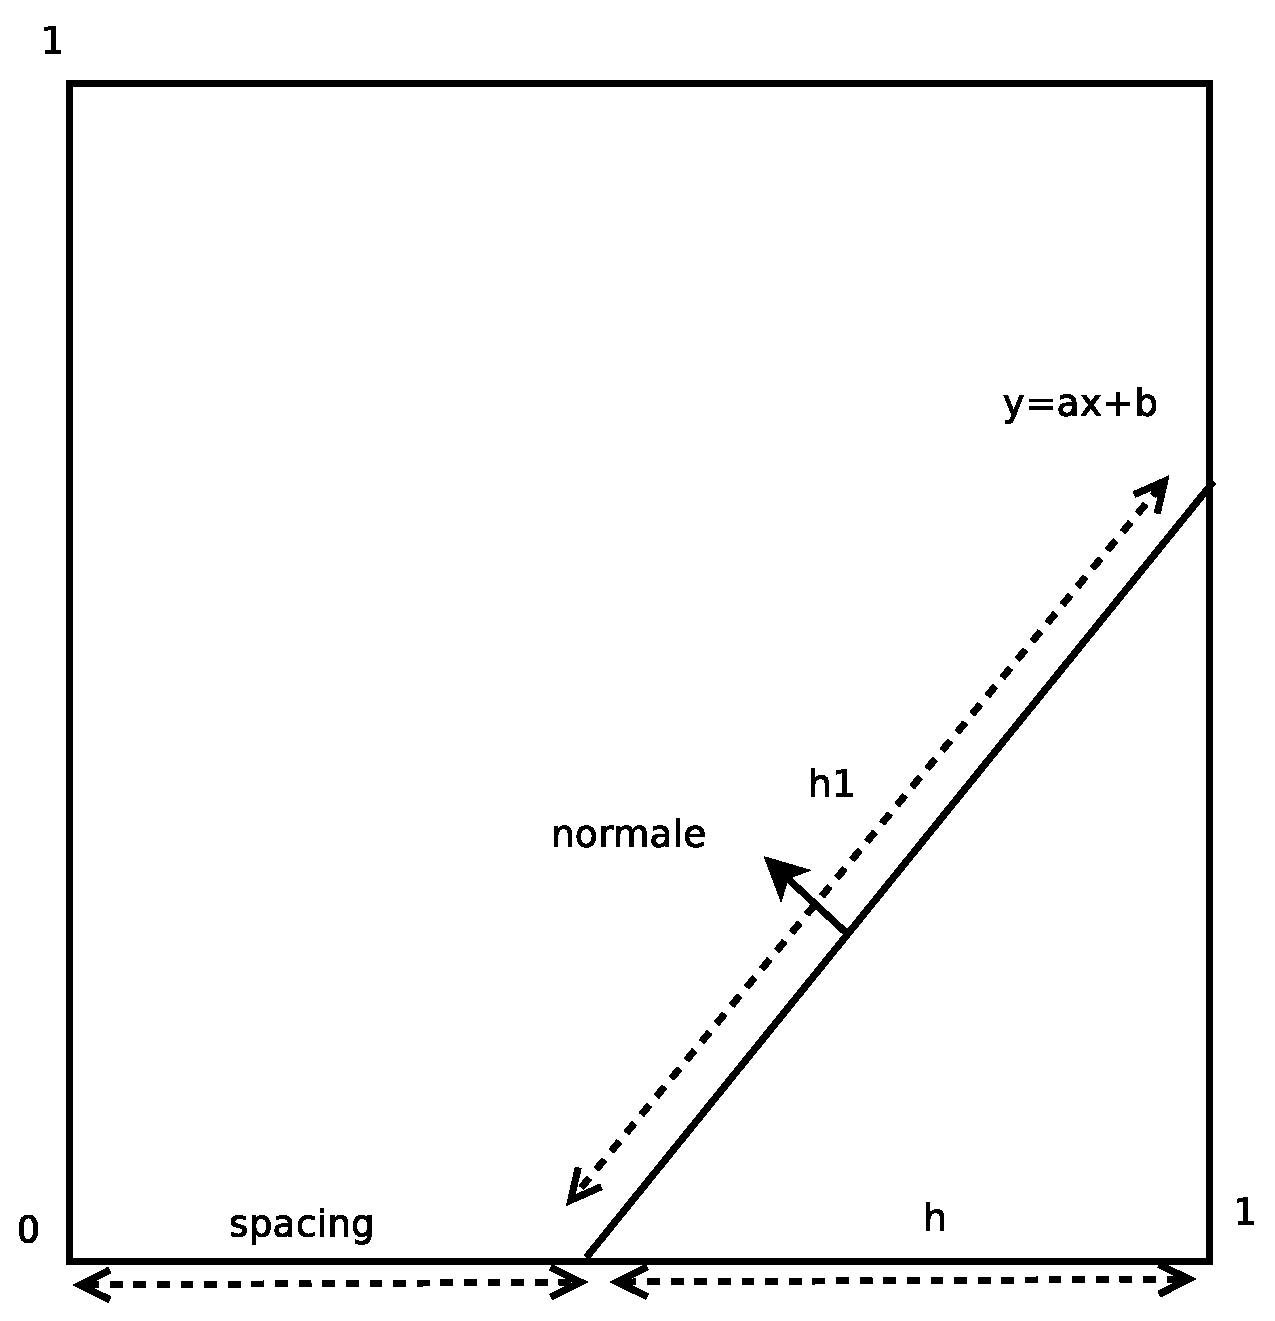
\includegraphics[width=0.65\textwidth]{img/cap2/mesh.eps}
\caption{Principali parametri di definizione per una frattura}
\end{center}
\end{figure}

\begin{Code03_01}[caption={Definizione della frattura}]
[fractureData]

spaceDimension = 1.

   [./levelSet]		// parametri di definizione del level set
     // funzione level set che rappresenta la frattura
     levelSet = y-a*x-b 			
     ylevelSet = y-a1*t-b1 			
     xlevelSet = x-a2*t-b2				          
     levelSetCut = -1	
     yMap = a1*t+b1					
     xMap = a2*t+b2				
     // fattore di scala, rapporto tra la lunghezza della mesh di integrazione e la 
     // lunghezza della mesh reale
     jacMap = [ h/h1 ]				
     normalMap = [ ]					
     integrationTypeSimplex = IM_STRUCTURED_COMPOSITE(IM_TRIANGLE(3),1)
   [../]

   [./domain]		// parametri di definizione del dominio di integrazione
     thickness = 
     spacing = x+c      	
     spatialDiscretization = n
     // dimensioni del dominio
     translateAbscissa = c
     lengthAbscissa = h1
     lengthOrdinate = 0.
     lengthQuota = 0.
     meshType = GT_PK(1,1)
     // variabili per l'integrazione
     integrationTypeVelocity = IM_GAUSS1D(3)
     integrationTypePressure = IM_GAUSS1D(2)		
     FEMTypeVelocity = FEM_PK(1,1)
     FEMTypePressure = FEM_PK(1,0)
     FEMTypeLinear = FEM_PK(1,1)
   [../]

   [./darcy]		// parametri per la definizione del problema di Darcy
     etaNormal = 0.01
     etaNormalDistribution = 1. 
     etaTangential = 100.
     etaTangentialDistribution = 1.
     source = 
     solution = 
     velocity = 
   [../]

[../]

\end{Code03_01}

